\section*{Exercice 134 -- Correcteur P}
\setcounter{exo}{0}
% POLE CB JC
On considère un asservissement à correction proportionnelle décrit par le schéma-bloc à retour unitaire de la
figure ci-dessous.

\begin{center}
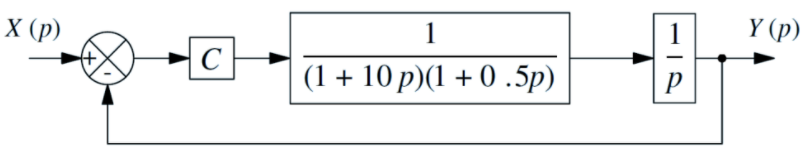
\includegraphics[width=\linewidth]{084_01}
\end{center}



\subparagraph{}
\textit{Indiquer, en justifiant la réponse, à quelle fonction de transfert correspondent les diagrammes de
Bode de la figure ci-dessous.}
\ifprof
\begin{corrige}
\end{corrige}
\else
\fi

\begin{center}
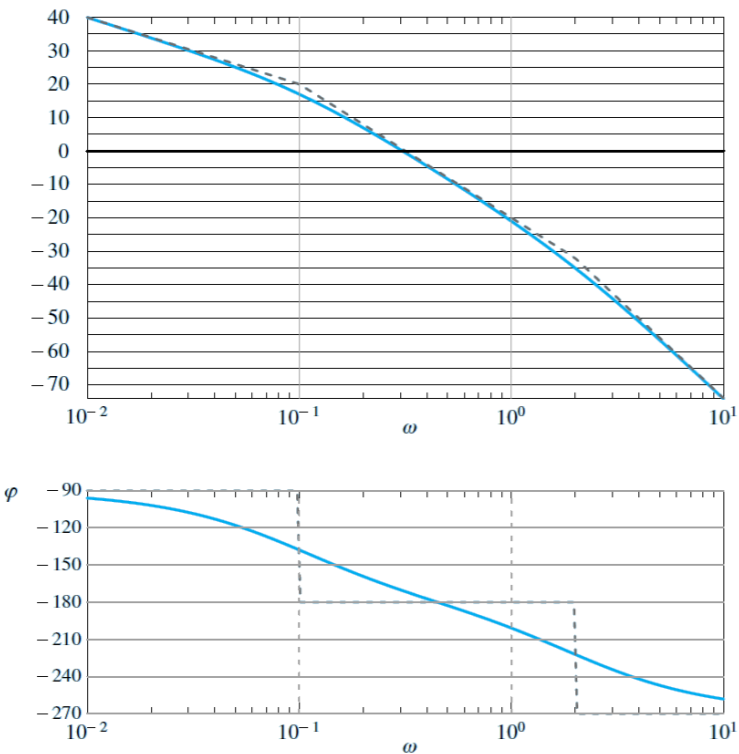
\includegraphics[width=\linewidth]{084_02}
\end{center}


\subparagraph{}
\textit{Déterminer graphiquement les marges de gain et de phase du système décrit précédemment dans le
cas où $C=1$.}
\ifprof
\begin{corrige}
\end{corrige}
\else
\fi


\subparagraph{}
\textit{Le cahier des charges impose des marges de gain et de phase minimales de \SI{12}{dB} et \SI{40}{\degres}. Déterminer graphiquement la plus grande valeur de $C$ permettant de vérifier ce cahier des charges.}
\ifprof
\begin{corrige}
\end{corrige}
\else
\fi

La figure ci-dessous donne l’évolution temporelle de la sortie du système lorsqu’il est soumis à une entrée
en échelon.

\begin{center}
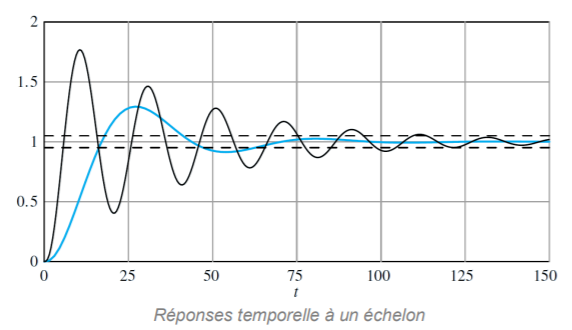
\includegraphics[width=\linewidth]{084_03}
\end{center}

\subparagraph{}
\textit{Indiquer, en le justifiant, qu’elle est la courbe qui correspond au système non corrigé et quelle est la
courbe qui correspond au système corrigé.}
\ifprof
\begin{corrige}
\end{corrige}
\else
\fi

